\section{Asset Identification Technologies}

For the purposes of this project, an \enquote{asset
  identification technology} refers to any technology suited
to identifying as asset; i.e., scanning items at a
supermarket till with \hyperref[ss:barcodes]{barcodes},
using \hyperref[ss:nfc]{NFC} to pay for shopping using
contactless payment, or protecting said items against theft
using \hyperref[ss:rfid]{RFID}-based security tags.

\subsection{Barcodes} \label{ss:barcodes}

\glsdisp{barcode}{Barcodes} have been used in shops to
identify products
since 1974, designed to transfer data more quickly and
reliably and eliminate human error when identifying assets
\parencite{whatIsABarcode}.

Originally, barcodes were exclusively one-dimensional (1D),
composed of vertical lines arranged horizontally to
represent alphanumeric data.
1D barcodes are still abundant today; retail uses
the Universal Product Code (UPC) and European Article
Numbers (EAN) standards, and logistics uses Code 128.
To aid with scanning, margin on the left and right sides
can be added, named a \enquote{quiet zone}.
Some standards also employ a \enquote{guard pattern}:
specific markings at the start and end of a barcode to
indicate so \parencite{whatIsABarcode}.

As scanning technology has improved, so have barcodes.
Two-dimensional barcodes contain information horizontally
and vertically, thus storing more data relative to their
size.
See Figure~\ref{fig:barcodes} for an example of each.
Common standards include QR codes, used in automotive and
commercial marketing applications, and Aztec codes, used
for mobile ticketing \parencite{whatIsABarcode}.
As well as a quiet zone, 2D barcodes require a finder
pattern and a clocking pattern: 

\begin{displayquote}
  The finder pattern is the L-shaped
  pattern located around the outside edge of two sides of the
  2D code.
  This is used to ensure proper orientation during decoding.
  Opposite the finder pattern is the clocking pattern, a
  series of alternating black and white cells that define how
  big a single cell is and the size of the code (number of
  rows and columns) for decoding.
  The quiet zone is similar to that of 1D barcodes; for 2D
  codes, however, it must surround the entire code
  \parencite{whatIsABarcode}.
\end{displayquote}

\begin{figure}[h]
  \centering
  \begin{subfigure}{\subfigwidth}
    \centering
    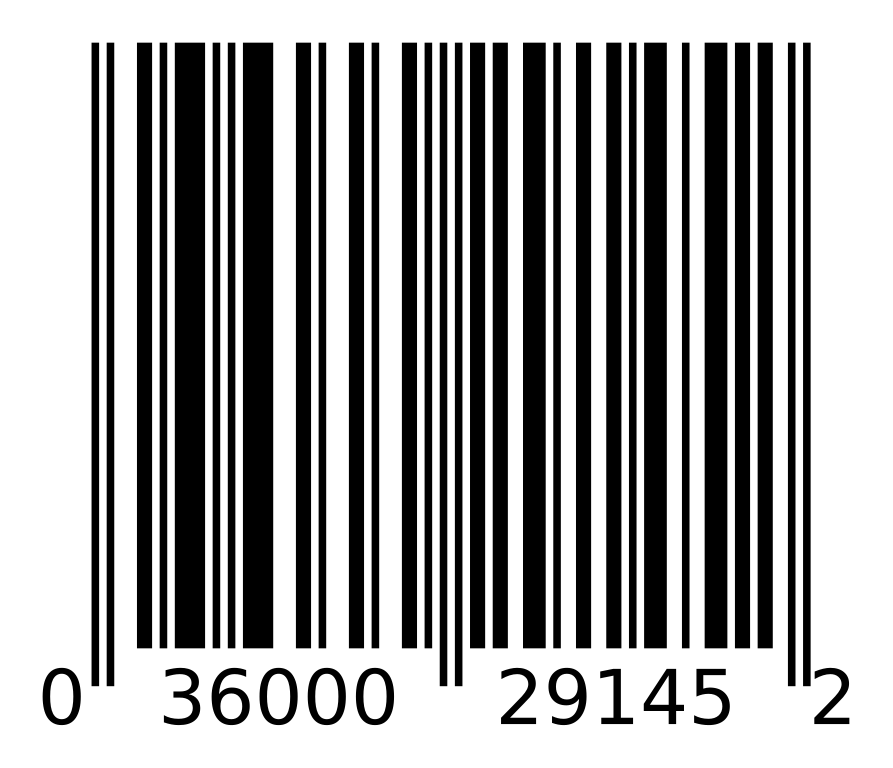
\includegraphics[height=0.4\linewidth]{04
      research/assets/upc barcode.png}
    \caption{UPC Barcode (1D)}
    \parencite{img:upcBarcode}
  \end{subfigure}
  \begin{subfigure}{\subfigwidth}
    \centering
    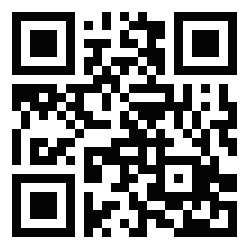
\includegraphics[height=0.4\linewidth]{04
      research/assets/qr code.jpg}
    \caption{QR Code (2D)}
    \parencite{img:qrCode}
  \end{subfigure}

  \caption{Barcode Standards}
  \label{fig:barcodes}
\end{figure}

Although dedicated hardware is produced for barcode
scanning, it is absolutely not required due to minimal
computational requirements and the public availability of
exceedingly common standards such as Quick Response (QR)
\parencite{qrCodeStandard}.
\cite{androidBarcodeScanner} demonstrates a barcode scanner
for Android as far back as 2009.

In researching scanning errors and equipment failures of
barcoding, \cite{barcodeRfidComparison} identified some
issues: 

\begin{itemize} 

  \item \enquote{Unreadable labels} --- a barcode is only as
        durable as the material onto which it is printed/screen on
        which it is displayed 

  \item \enquote{Broken scanning equipment} --- an issue
        inherent to technology 

\end{itemize} 

\subsection{RFID} \label{ss:rfid} 

A system using \gls{rfid} consists of a \enquote{reader}
device and a number of \enquote{transponders} (transmitter
and responder).
RFID is used for goods tracking in logistical contexts and
goods surveillance in shops \parencite{whatIsRfid}.

Fundamentally, all transponders have an antenna to
send/receive signals to a reader, microchip to store data.
Passive transponders also feature a capacitor, which
receives power from the reader via induction.
Active transponders are batteries-included, thus not
requiring induction which allows electromagnetic waves to
\enquote{couple} with the reader \parencite{whatIsRfid}.

Another aspect of an RFID system is signal frequency.
Refer to Table~\ref{tbl:rfidFreq} for a comparison, adapted
from \cite{whatIsRfid}.

\begin{table}[ht]
  \centering
  \begin{tabular}{lcccc}
    & \multicolumn{4}{c}{Frequency} \\ \hline

    & Low & High & Ultra-high & Super-high \\ \hline

  \makecell[l]{Frequency\\range} & Under 135kHz & 13.56 MHz & \makecell{868 MHz (EU)\\915 MHz (USA)} & \makecell{2.45 GHz, \\ 5.8 MHz} \\

  Wave & Radio wave & Radio wave & Radio wave & \makecell{Radio wave/\\microwave} \\

  \makecell[l]{Method of\\coupling} & Inductive & Inductive & Electromagnetic & Electromagnetic \\

  Range & Up to 1m & Up to 3m & 10--100m & 3--300m \\

  \makecell[l]{Transmission\\rate} & Low & High & High & Very high \\

  \makecell[l]{Disrupted by\\liquid} & Low & Low & Very high & Very high \\

  \makecell[l]{Disrupted by\\metal} & Yes & Yes & No & No \\

  \makecell[l]{Requires\\line of sight} & No & No & Partial & Yes \\
\end{tabular}

  \caption{Comparison of RFID frequencies}
  \label{tbl:rfidFreq}
\end{table}

\cite{barcodeRfidComparison} also identified issues present
in an applied RFID system:

\begin{itemize}

  \item \enquote{Misread tags} --- a perfect
        connection is virtually impossible

  \item \enquote{Broken RFID and tag equipment}
        --- again, an issue inherent to technology

\end{itemize}

\subsection{NFC} \label{ss:nfc}

Because \gls{nfc} is not a single standard, rather a set of
standards, its operation at a technical level cannot be
explained in general terms.

At a functional level, NFC is fast becoming an abundant
technology in mobile devices like
\hyperref[ss:biometrics]{biometrics}; 90\% of new phones
are NFC-enabled \parencite{nfcHandsetStats}.
Devices must be within a few centimetres to communicate.
The wireless connection transfers data up to 424Kbps, also
compatible with Wi-Fi and Bluetooth \parencite{nfc}.
Ultimately, it has an extensive range of applications as
identified by \cite{nfc}: 

\begin{itemize} \item Contactless payments on mobile
        devices (e.g., \cite{androidPayWithPhone, applePay}) \item
        Electronic ticketing for transportation (e.g.,
        \cite{digitalTickets}) \item Device pairing \item
        Access/inventory control \end{itemize} 

\subsection{Conclusions} 

With its huge span of ranges, RFID has good potential to
integrate with the identification methodology.
Nonetheless, its proprietary hardware requirements conflict
with the \hyperref[ss:goal]{desired flexibility}.

Both barcodes and NFC have hardware requirements: a camera
and an NFC implementation respectively.
Due to the versatility of barcodes and the scale of
camera-equipped devices (e.g., PCs with webcams, laptops,
tablets, smartphones), they are the best option for the
identification methodology.
